\section{Architecture} % (fold)
\label{sec:implementation}

% TXODO: intro:
% de richting dit hoofdstuk nu op gaat zou ik een intro geven met wat en hoe je het gaat doen en dan mpls en openflow vergelijken met het implementeren van de requirements van het foorgaande hoofdstuk...
% 
% niet zeggen , as defined in section 2, maar in introductie suidelijk maken dat je gaat kijken naar hoe je dvpns kunt maken in mpls en openflow, 
% 
% in related work kun je dan een vergelijking maken met andere technologieen...
% 
% dus, pbb weg, naar related work... alleen mpls openflow en de comparison in dit hoofdstuk

This section will first describe the technical details of \ac{mpls} with regards to the features required for implementing \acp{dvpn}. We will design an architecture to implement this service and point out the limitations. 
Next, we will describe the \ac{sdn} architecture and the OpenFlow specification. Also looking at the features they provide to implement a \ac{dvpn} service.
In Appendix~\ref{sub:spb} we have also taken a look at \ac{atm} and \ac{spb}, both are technologies that can be used to implement \acp{vpn} but are missing key requirements to support \acp{dvpn}.

\subsection{\acs{mpls}} % (fold)
\label{sub:mpls}

\ac{mpls} is known for its scalability and extensibility. Over the past decade additions have been made to the original specification to overcome a plethora of issues within carrier networks. This initially started with trying to implement fast forwarding in legacy switches using labels (or tags) at the start of the frame \cite{tag-switching}. When this issue became surmountable using new hardware, \ac{mpls} had already proven to be capable of transporting a wide arrange of protocols on the carrier backbone network, all the while also providing scalability, \ac{te} and \ac{qos} features to the operators.

\ac{mpls} itself is a technology for forwarding frames through the network, does not provide any additional functionalities such as topology discovery, route determination, resource management, etc. These functions are left to a stack of other protocols. Without \ac{ip} reachability throughout the network these protocols cannot exchange traffic and so, as a prerequisite, \ac{mpls} relies on an \ac{igp} like \ac{ospf} to discovery the topology.

The distribution of labels has to be facilitated as well, which is done using \ac{ldp} and/or \ac{rsvp}. These protocols run between each device in the path between two \acp{pe} and exchange the labels that the will assign to a certain path, thereby setting up a \ac{lsp}. The labels assigned are always of `local significance,' meaning that the \ac{p}/\ac{pe} device that needs to forward the labels, will announce its own chosen labels. The \ac{ldp} protocol does this by distributing its labels from the egress \ac{pe} up towards the ingress \ac{pe} based on \ac{igp} costs. \ac{rsvp}, on the other hand, signals its paths from the ingress \ac{pe} towards the downstream \ac{pe} based on constraints, potential explicit hops or as a last resort using the \ac{igp} next hop. Label distribution is still determined from egress to ingress, but the actual path is determined at the head-end. To determine the best path to take, \ac{rsvp} uses the \ac{cspf} algorithm which can take into account link characteristics like bandwidth or \ac{frr} support. This allows \ac{rsvp} \acp{lsp} to take more well informed paths through the network and together with support for defining explicit paths, allows for granular \ac{te} features which \ac{ldp} lacks. Both \ac{ldp} and \ac{rsvp} also allow for the use of multiple paths over the network to share traffic load towards a \ac{pe}.

The \ac{frr} feature is unique to \ac{rsvp} and provides the network with fast failure recovery. It does so by preprovisioning a so-called backup \ac{lsp} next to the primary \ac{lsp}. When a failure is detected on the primary \ac{lsp}, traffic is immediately shifted towards the standby path, yielding a sub-50ms failover. Obviously, this value also depends on the time it takes for the failure to be detected. Therefore it is important to have some sort of detection mechanism in place. One that is commonly used and integrates with \ac{ospf} is \ac{bfd}. This protocol sets up sessions between devices and triggers an alarm when the session does not behave as expected. At which point \ac{frr} swaps the traffic to the preprovisioned backup path. To differentiate traffic coming from a normal, `protected' path and traffic taking a `detour' path, \ac{frr} adds another \ac{mpls} tag to the \ac{mpls} label stack.

\acp{vpn} are also provided by additional protocols. Layer 3 \acp{vpn} make use of \ac{bgp} to distribute client prefixes to the edges of the carrier network. The core is only concerned with the forwarding of labels and has now knowledge of these \acs{ip} prefixes. Layer 2 \acp{vpn} make use of \ac{vpls}, a service which encapsulates the entire Ethernet frame and pushes a label to it to map it to a certain separated network. Again, the core is only concerned with the labels and only the edges need to know the clients \acs{mac} addresses. When setting up a \ac{vpls} instance (a \acp{vpn}), \ac{ldp} sessions are setup between all \acp{pe} part of the same \ac{vpls} instance. Consecutively, the \acp{pe} will exchange their chosen labels for that instance between each other.

The \acp{cmac} in a \ac{vpls} instance are normally learned through the data plane. That is, when a frame comes in from a \ac{ce}, the \ac{pe} learns the \ac{sa} behind the corresponding port. If it doesn't know the \ac{da}, it will flood the frame to other \acp{pe} with member ports in that instance. These \acp{pe} in turn learn the \ac{sa} as well behind the ingress \ac{pe}. This is also illustrated in Figure~\ref{fig:vpn-traffic}. When a large number of \acp{cmac} are present within a \ac{vpls} instance this can cause a lot of broadcast traffic, specifically \ac{arp} traffic. To solve this, the \ac{evpn} standard has been proposed \cite{evpn}. This technique provides \ac{mac} learning in the control plane by exchanging learned \acp{cmac} between \acp{pe} using Multi-Protocol \ac{bgp}. Additionally it learns the \ac{ip} addresses associated with the \acp{cmac} and distributes those to other \acp{pe}. The \acp{pe} are thereby able to act as an \ac{arp} proxy, as illustrated in Figure~\ref{fig:arp-proxy}.

\begin{figure}[!h]
	\centering
	\begin{subfigure}[b]{0.3\textwidth}
		\centering
		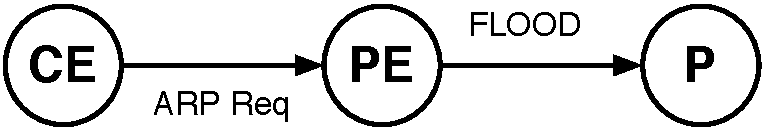
\includegraphics[width=\textwidth]{./includes/arp-no-proxy.pdf}
		\caption{Normal \acs{arp} Request.}
		\label{fig:arp-no-proxy}
	\end{subfigure}\hspace*{1cm}
	\begin{subfigure}[b]{0.3\textwidth}
	\centering
		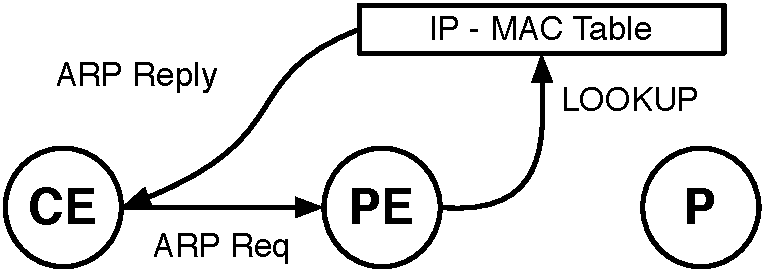
\includegraphics[width=\textwidth]{./includes/arp-proxy.pdf}
		\caption{\acs{arp} proxy in \ac{pe}.}
		\label{fig:arp-proxy}
	\end{subfigure}
	\caption{Processing of \acs{arp} requests at the \ac{pe}.}
\end{figure}

The different protocols all depend on each other, as illustrated in Figure~\ref{fig:mpls-stack}. Each \ac{pe} device runs this stack, while \ac{p} devices run a subset which is shaded. 

\begin{figure}[!h]
	\centering
	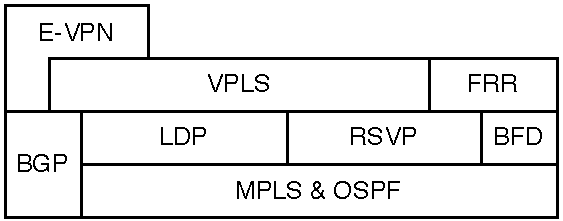
\includegraphics[width=7cm]{./includes/mpls-stack.pdf}
	\caption{Dependency stack of \ac{mpls}-related technologies.}
	\label{fig:mpls-stack}
\end{figure} 

To configure a \ac{dvpn} using \ac{mpls} first the participating \acp{pe} need to be configured with the new \ac{vpls} instance to which the member \ac{ce} ports will be added. Next, constraints are defined by the \ac{nms}, which can be in the form of an explicit route to make a static route or by defining loose constraints based on bandwidth limits which can be used the \ac{cspf} algorithm. Using these constraints, paths are installed at each \ac{pe} towards every other participating \ac{pe}. These paths are then added to the \ac{vpls} instance, allowing \ac{ldp} sessions to be setup between the \acp{pe}. Next, for \ac{frr}, backup \acp{lsp} need to defined similarly to the primary \ac{lsp} but over a different path, which can again be done using constraints to exclude the other links. Utilization of the links in the network has to be monitored as well and when a path has a link which is nearing capacity, new \acp{lsp} have to be provisioned and some \ac{vpls} paths move to those \acp{lsp}. And finally the ingress traffic on the \ac{ce} ports need to be rate limited. This procedure is not standardized and is dependent on support of the hardware.

The procedure above implies that the backbone network has been setup with the following protocols and features already enabled: \ac{ip} addressing, \ac{ospf} routing, \ac{mpls} forwarding, \ac{rsvp} with \ac{frr} and \ac{bfd}. After initial setup of the backbone network the \ac{nms} is only concerned with the \acp{pe}, as can also be seen in Figure~\ref{fig:nms-stack}. However, the \ac{nms} needs to be aware of the \acp{pe} it needs to consult, the intermediate \acp{p} if it wants to use \ac{te}, the network resources in the path and of course the actual member ports.

Implementing \acp{vpn} using \ac{mpls} has been shown to be possible using the protocols that have been engineered to provide all the required features. The technologies are built upon each other instead of being evolved upon. This causes their dependencies to grow more complex over time which in turn makes it difficult for the \ac{nms} to deal with all the different protocols. Additionally, developing and maintaining an efficient \ac{nms} is also more difficult due to the lack of a common abstracted interface to the network devices.

\begin{figure}[!h]
	\centering
	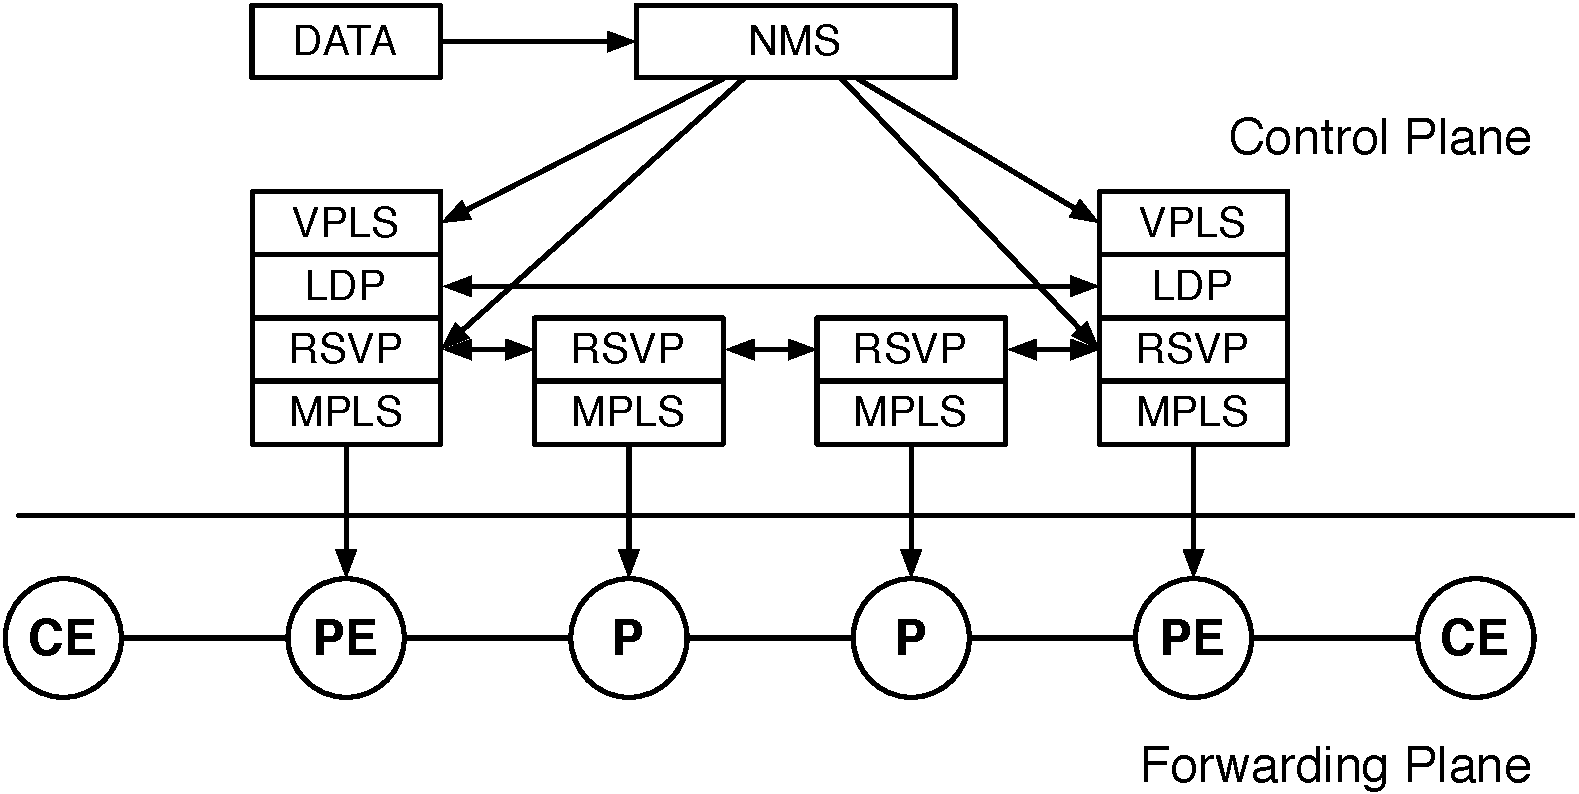
\includegraphics[width=10cm]{./includes/nms-stack.pdf}
	\caption{Provisioning a \ac{dvpn} using \ac{mpls}.}
	\label{fig:nms-stack}
\end{figure}

% subsection mpls (end)

\subsection{OpenFlow} % (fold)
\label{sub:openflow}

%Section~\ref{sec:introduction} gave a short introduction into what \ac{sdn} and OpenFlow entail and what it promises in terms of cost savings and agility. 
\acl{sdn} is the general principle of designing flexible networks using open interfaces towards the hardware. OpenFlow is a subcomponent of this new principle which provides a protocol between the forwarding plane of the networking devices and a centralized controller. A general overview of the \ac{sdn} architecture and OpenFlow is given in Figure~\ref{fig:of-arch}. OpenFlow provides the controller with an \ac{api} that can be used to install flow entries directly in the forwarding plane of the devices. Flow entries consist of six fields:

\begin{description}[leftmargin=!,labelwidth=\widthof{\bfseries Instructions}]
	\item[Match] This field contains a list of frame/packet characteristics that will need to be present to match to this entry, e.g.\ \ac{da}, \ac{ip} source address or \ac{mpls} tags.
	\item[Priority] The precedence of this flow entry over other flow entries to which a certain frame matches.
	\item[Counters] Frames matching to this entry are counted for monitoring purposes.
	\item[Instructions] When a frame is matched using the match field, it is processed according to a list of instructions, which may include forwarding out of a port, rewriting headers and/or applying meters.
	\item[Timeouts] The time that a flow entry can be live until it is discarded.
	\item[Cookie] Value assigned by controller to identify the flow (not used to forward frames).
\end{description}

\begin{figure}[!h]
	\centering
	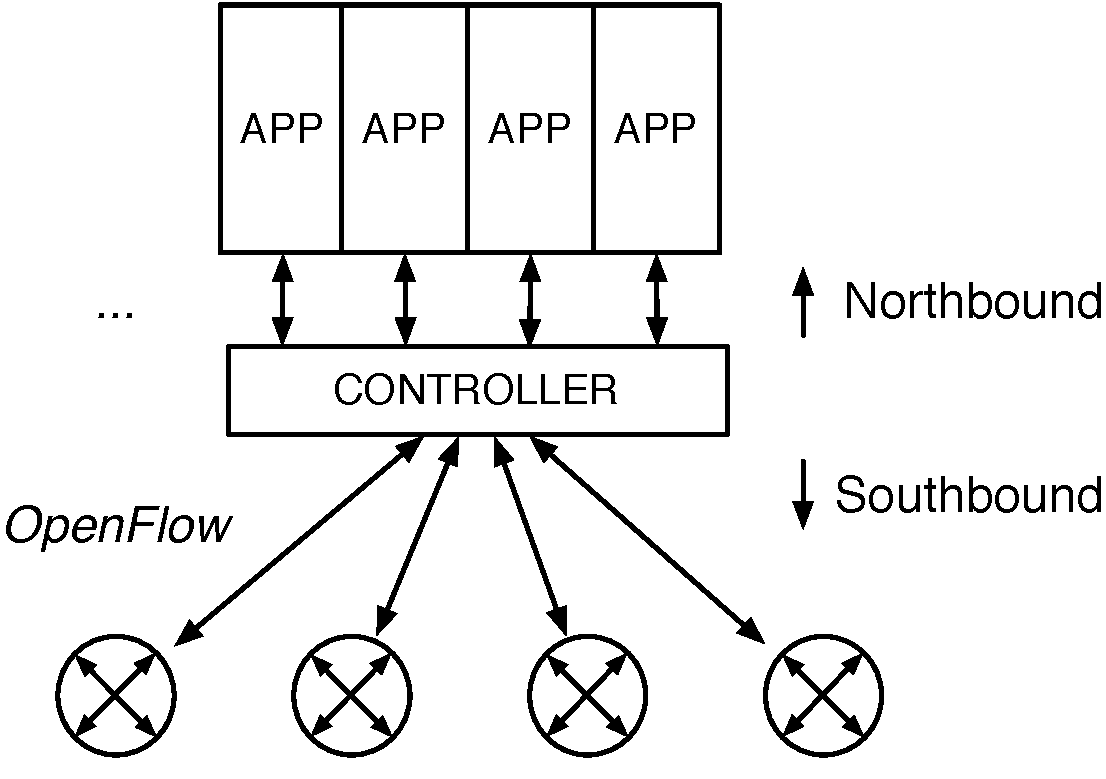
\includegraphics[width=7cm]{./includes/of-arch.pdf}
	\caption{Architecture of \ac{sdn} and OpenFlow.}
	\label{fig:of-arch}
\end{figure}

The frame fields that can be matched upon have changed over the lifetime of the OpenFlow specification. For example, version 1.0 could only match and/or act upon tagged traffic using a single outer-\acs{vlan} tag. Version 1.1 added matches and actions for Q-in-Q tags and \ac{mpls} labels, and version 1.3 could also match \ac{pbb} tags. See Table~\ref{tb:of-versions} for a comparison of key features in different versions of OpenFlow spec. 

%\begin{table}[!h]
%	\centering
%	\begin{tabular}{r|cccc}
%	 			& 1.0 & 1.1 & 1.2 & 1.3 \\
%	\hline
%	VLAN Tags 	& \checkmark & \checkmark & \checkmark & \checkmark \\
%	Q-in-Q Tags &   & \checkmark & \checkmark & \checkmark \\
%	MPLS Tags 	&   & \checkmark & \checkmark & \checkmark \\
%	PBB Tags 	&   &   &   & \checkmark \\
%	Groups 		&   & \checkmark & \checkmark & \checkmark \\
%	Rate limiting & \checkmark & \checkmark & \checkmark & \checkmark  \\
%	\end{tabular}
%	\caption{Comparison of OpenFlow versions regarding key features for \acp{dvpn}.}
%	\label{tb:of-versions}	
%\end{table}

Note that rate limiting on a per port basis has been available in OpenFlow since version 1.0. Additionally, version 1.3 added support for per flow rate limiting using so called `meters' which can be assigned to specific flows. By doing so it becomes possible to also rate limit flows on certain aggregation ports rather than just at the ingress port of the \ac{ce}.

The installation of flow entries is done by the controller, governed by the applications running on it. Applications can be written to provide functions like topology discovery, routing, etc. Moreover, without these installed applications, the network will be unable to forward any traffic. The interface between the applications and the controller is also being referred to as the `northbound interface'. This interface, in contrast to the southbound OpenFlow interface, has not been specified and varies between different controller implementations, limiting the portability of the network applications.

Unlike contemporary technologies that require inter-device communication before any paths can be set up, the forwarding tables of OpenFlow devices are empty. The only prerequisite is that the devices all have a management connection to the controller from which they can receive their forwarding information.

The controller is the combination of hardware and software components that are preferably setup redundantly and share a complete view of the network, which they share with the applications running on it. To provide the network and its control with redundancy in case of failures, the `controller' component can refer to a logical controller entity, not specifically a single physical server. However, the actual design and implementation of such a system is beyond the scope of this paper.

Current OpenFlow versions are not yet supported by all controllers. We are inspecting version 1.3.1 of the specification which supports the features described. However, at the time of writing there are only two controllers supporting the 1.3 version:
\begin{itemize}
	\item Ryu by NTT \cite{ryu}, and
	\item NOX extensions by CPqD research center from Brazil \cite{cpqd}.
\end{itemize}
The controller developed under the OpenDaylight project lacks support for version 1.3.

Implementing \acp{dvpn} using OpenFlow relies mostly on the applications running on the controller. When they are written and configured as desired, provisioning a \ac{dvpn} would only require the input of the data. After which the applications and controller install flow entries into all the network devices in the \ac{dvpn} path, as can be seen in Figure~\ref{fig:nms-stack-of}.

\begin{figure}[h]
	\centering
	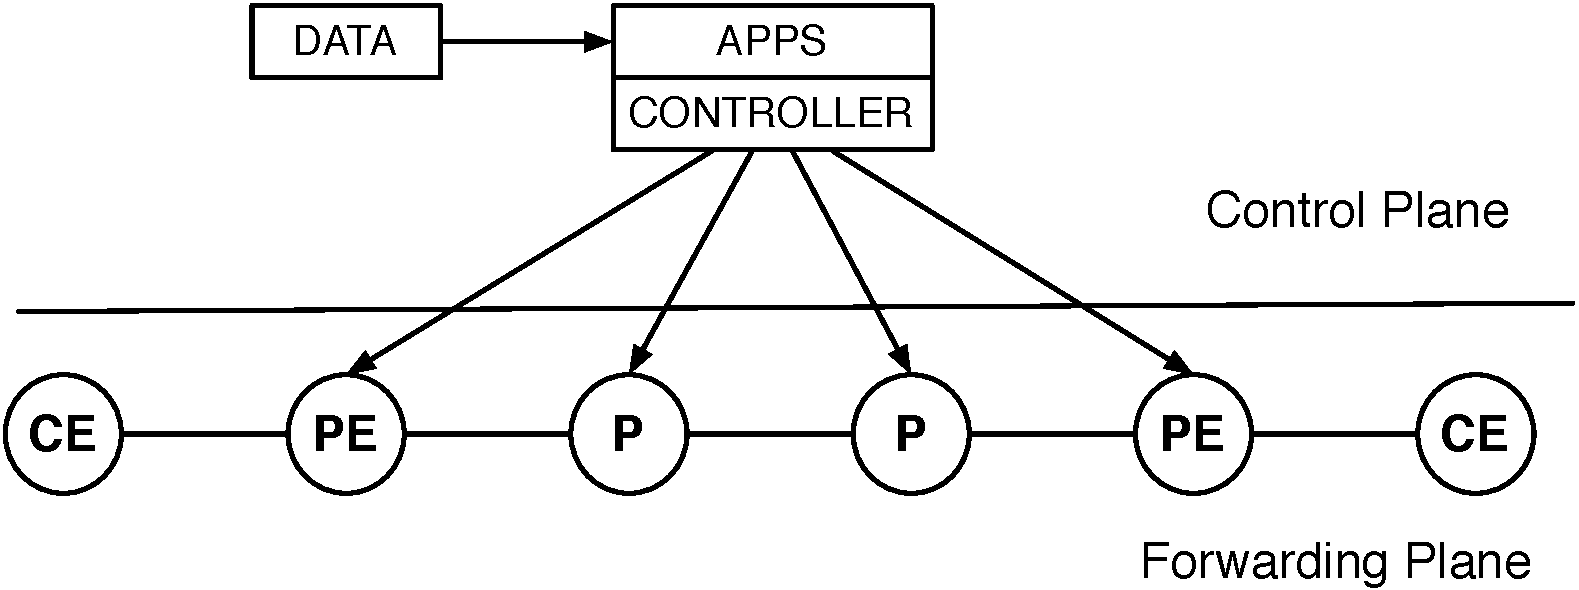
\includegraphics[width=10cm]{./includes/nms-stack-of.pdf}
	\caption{Provisioning a \ac{dvpn} using OpenFlow.}
	\label{fig:nms-stack-of}
\end{figure}

\subsubsection{\acs{dvpn} Provisioning} % (fold)
\label{ssub:dvpn_application}

To implement \acp{dvpn}, one or more applications providing the functions analogous to contemporary implementations need to be implemented in the OpenFlow setup:

\begin{description}[leftmargin=!,labelwidth=\widthof{\bfseries Topology Discovery}]
	\item[Topology Discovery] Network devices do not require \ac{ip} connectivity between each other to exchange route information. Instead, they rely on their connection to the controller to provide them with information. A topology discovery application will instruct network devices to send out unique discovery messages which are then received by other devices, which forward the message back up to the controller. By keeping information on which packet goes in and comes out where, the application can get an overview of the network. By centralizing the topology discovery process, network operators can benefit from more efficient synchronization and faster convergence.
	
	\item[\ac{dvpn} Provisioning] The \ac{dvpn} input will provide the application with at least the \ac{ce} port and preferably the corresponding \ac{mac} and/or \ac{ip} address. It can then instruct the path provisioning component to set up paths between all the \acp{pe} participating in the \ac{dvpn}. 
	
	\item[Path Provisioning] Using the discovered topology, paths are setup over those routes between \acp{pe} with member \ac{ce} ports in a common \ac{dvpn}. This means that the flow entries are installed proactively in the \acp{p} and \acp{pe} when a \ac{dvpn} is setup. Instead of waiting for one of them to send a message to the controller asking what to do with an unknown incoming frame, this proactive approach allows for better scalability (less requests to the controller) and faster initial forwarding (no buffering while consulting controller).

	\item[\acs{oam}] The controller and applications provide a complete overview of the network but troubleshooting and monitoring still has to be done at the network level as well. Different approaches can be taken to do so, one of which could be sending out periodic keep-alive messages in the same path from the controller down to the ingress \ac{pe} that the egress \ac{pe} should forward back up to the controller. Another example is implementing an already defined \ac{oam} protocol in OpenFlow, as has been done in \cite{of-oam} which implemented Ethernet 802.1ag \ac{oam}.
	
		\item[Traffic Engineering] The path setup procedure uses data from the \ac{dvpn} input and the discovered network resources to provide the most optimal path between two \acp{pe}. Constraints for the paths taken by each \ac{dvpn} can be configured by the operator and influence the route selection directly over the whole platform. Also, using input from the \ac{oam} monitoring applications paths may be preferred or deprecated based on their performance.
	
	\item[\ac{cmac} Filtering] This application is concerned with keeping the provided or dynamically learned \ac{mac} addresses up-to-date. Additionally, a flow can be installed matching on the \ac{arp} EtherType that sends the \ac{arp} request towards the controller. If the application also keeps track of the \ac{ip} addresses of the \acp{ce} it can then act as an \ac{arp} proxy and reply to the requesting \ac{ce} with the correct \ac{ip} address.
\end{description}

Fast failover and \ac{ecmp} can be accomplished using the port `groups', which are available since version 1.1. Groups can be defined as a destination in a flow entry and contains a list of ports. The type of group defines the action of the group: `\textbf{all}' sends the frame out the frame out of all ports in the group (broadcast/multicasting); `\textbf{select}' outputs it to one of the ports (providing \ac{ecmp}); `\textbf{indirect}' is a single port group which can be used by multiple flow entries (aggregation); and `\textbf{fast failover}' which choses the first \textsl{live} port out of which it will forward the frame. To support `fast failover' a \textsl{liveness monitoring} technique needs to be implemented supported by the switch. However, apart from monitoring the state of the physical link, there has been no technique defined to monitor the liveness of inter-device links, such as \ac{bfd}. The same holds true for full path liveness monitoring which currently needs to be done using the controller, yielding a higher failure recovery time.

\begin{figure}[h]
	\centering
	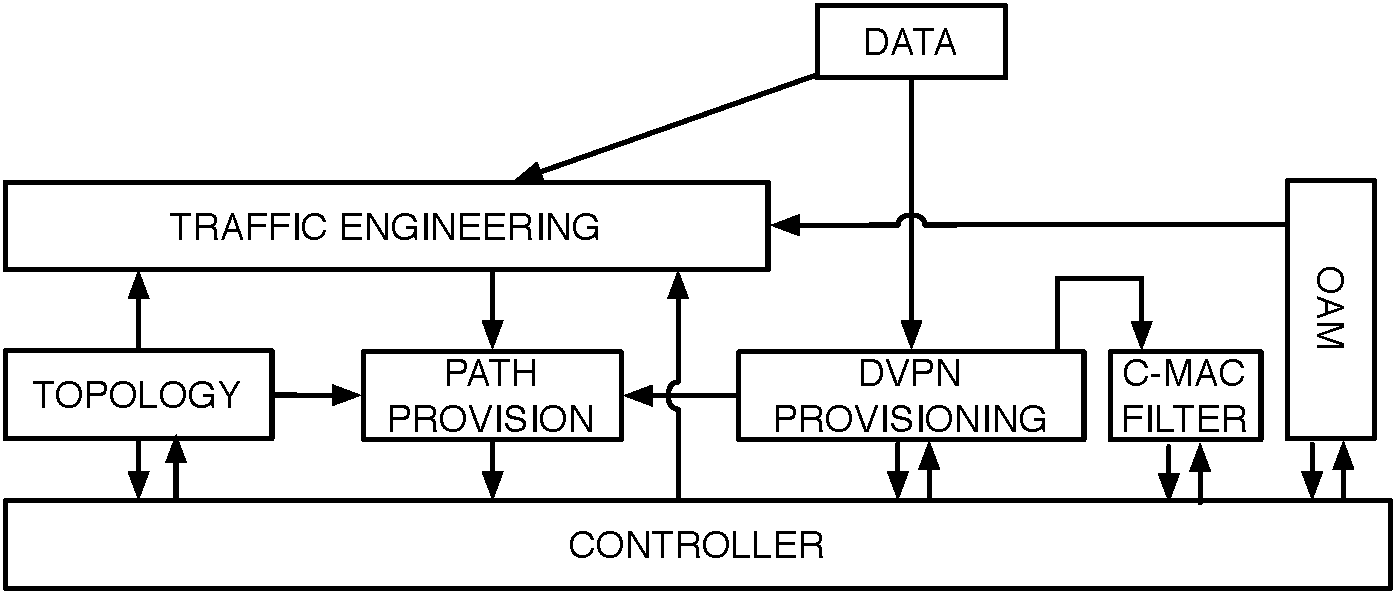
\includegraphics[width=10cm]{./includes/dvpn-apps.pdf}
	\caption{Interactions between application components to implement \acp{dvpn}.}
	\label{fig:dvpn-apps}
\end{figure}


The interaction between the different \ac{sdn} applications has been illustrated in Figure~\ref{fig:dvpn-apps}. Due to the abstractions introduced by the intermediate applications the \ac{nms} doesn't need to be aware of the network below. The applications will map the port member info from the \ac{nms} to the correct devices, and configure the \ac{dvpn}. Because of the abstractions and minimal initial configuration, adding extra hardware can also be taken care of without consulting the \ac{nms}: the applications will add it to the network and reroute traffic over the new device.



% subsubsection dvpn_applications (end)


% subsection openflow (end)

% section implementation (end)
